%!TeX root=../pridetop.tex
\chapter[Chapter \thechapter]{}
	
	\begin{figure}[t!]
\centering
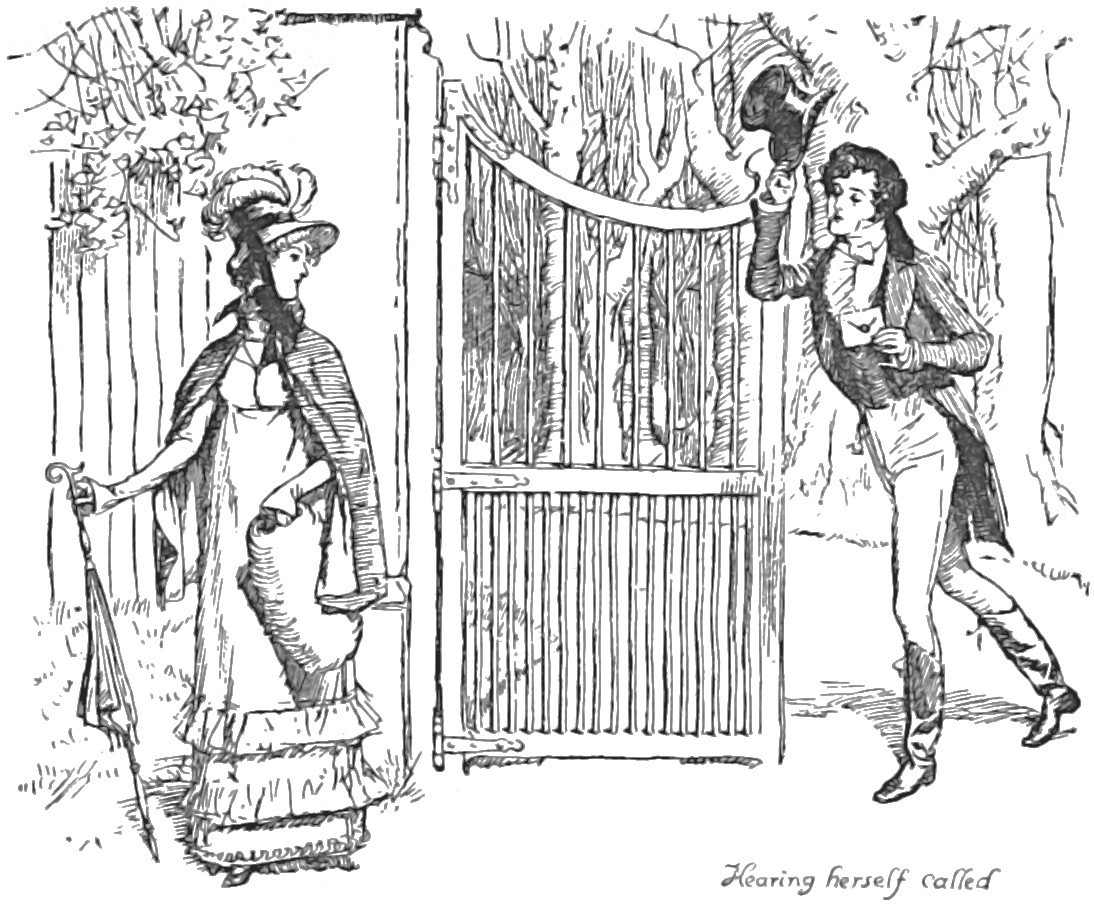
\includegraphics[width=\linewidth]{35top}
\captionlistentry{Headpiece to Chapter \thechapter}
\end{figure}


\lettrine[lines=6,image=true]{initials/chap35e}{lizabeth}  awoke the next morning to the same thoughts and meditations which had at length closed her eyes. She could not yet recover from the surprise of what had happened: it was impossible to think of anything else; and, totally indisposed for employment, she resolved soon after breakfast to indulge herself in air and exercise. She was proceeding directly to her favourite walk, when the recollection of Mr Darcy's sometimes coming there stopped her, and instead of entering the park, she turned up the lane which led her farther from the turnpike road. The park paling was still the boundary on one side, and she soon passed one of the gates into the ground.

After walking two or three times along that part of the lane, she was tempted, by the pleasantness of the morning, to stop at the gates and look into the park. The five weeks which she had now passed in Kent had made a great difference in the country, and every day was adding to the verdure of the early trees. She was on the point of continuing her walk, when she caught a glimpse of a gentleman within the sort of grove which edged the park: he was moving that way; and fearful of its being Mr Darcy, she was directly retreating. But the person who advanced was now near enough to see her, and stepping forward with eagerness, pronounced her name. She had turned away; but on hearing herself called, though in a voice which proved it to be Mr Darcy, she moved again towards the gate. He had by that time reached it also; and, holding out a letter, which she instinctively took, said, with a look of haughty composure, »I have been walking in the grove some time, in the hope of meeting you. Will you do me the honour of reading that letter?« and then, with a slight bow, turned again into the plantation, and was soon out of sight.

With no expectation of pleasure, but with the strongest curiosity, Elizabeth opened the letter, and to her still increasing wonder, perceived an envelope containing two sheets of letter paper, written quite through, in a very close hand. The envelope itself was likewise full. Pursuing her way along the lane, she then began it. It was dated from Rosings, at eight o'clock in the morning, and was as follows:—


Be not alarmed, madam, on receiving this letter, by the apprehension of its containing any repetition of those sentiments, or renewal of those offers, which were last night so disgusting to you. I write without any intention of paining you, or humbling myself, by dwelling on wishes, which, for the happiness of both, cannot be too soon forgotten; and the effort which the formation and the perusal of this letter must occasion, should have been spared, had not my character required it to be written and read. You must, therefore, pardon the freedom with which I demand your attention; your feelings, I know, will bestow it unwillingly, but I demand it of your justice.

Two offences of a very different nature, and by no means of equal magnitude, you last night laid to my charge. The first mentioned was, that, regardless of the sentiments of either, I had detached Mr Bingley from your sister,—and the other, that I had, in defiance of various claims, in defiance of honour and humanity, ruined the immediate prosperity and blasted the prospects of Mr Wickham. Wilfully and wantonly to have thrown off the companion of my youth, the acknowledged favourite of my father, a young man who had scarcely any other dependence than on our patronage, and who had been brought up to expect its exertion, would be a depravity, to which the separation of two young persons whose affection could be the growth of only a few weeks, could bear no comparison. But from the severity of that blame which was last night so liberally bestowed, respecting each circumstance, I shall hope to be in future secured, when the following account of my actions and their motives has been read. If, in the explanation of them which is due to myself, I am under the necessity of relating feelings which may be offensive to yours, I can only say that I am sorry. The necessity must be obeyed, and further apology would be absurd. I had not been long in Hertfordshire before I saw, in common with others, that Bingley preferred your elder sister to any other young woman in the country. But it was not till the evening of the dance at Netherfield that I had any apprehension of his feeling a serious attachment. I had often seen him in love before. At that ball, while I had the honour of dancing with you, I was first made acquainted, by Sir William Lucas's accidental information, that Bingley's attentions to your sister had given rise to a general expectation of their marriage. He spoke of it as a certain event, of which the time alone could be undecided. From that moment I observed my friend's behaviour attentively; and I could then perceive that his partiality for Miss Bennet was beyond what I had ever witnessed in him. Your sister I also watched. Her look and manners were open, cheerful, and engaging as ever, but without any symptom of peculiar regard; and I remained convinced, from the evening's scrutiny, that though she received his attentions with pleasure, she did not invite them by any participation of sentiment. If \textit{you} have not been mistaken here, \textit{I} must have been in an error. Your superior knowledge of your sister must make the latter probable. If it be so, if I have been misled by such error to inflict pain on her, your resentment has not been unreasonable. But I shall not scruple to assert, that the serenity of your sister's countenance and air was such as might have given the most acute observer a conviction that, however amiable her temper, her heart was not likely to be easily touched. That I was desirous of believing her indifferent is certain; but I will venture to say that my investigations and decisions are not usually influenced by my hopes or fears. I did not believe her to be indifferent because I wished it; I believed it on impartial conviction, as truly as I wished it in reason. My objections to the marriage were not merely those which I last night acknowledged to have required the utmost force of passion to put aside in my own case; the want of connection could not be so great an evil to my friend as to me. But there were other causes of repugnance; causes which, though still existing, and existing to an equal degree in both instances, I had myself endeavoured to forget, because they were not immediately before me. These causes must be stated, though briefly. The situation of your mother's family, though objectionable, was nothing in comparison of that total want of propriety so frequently, so almost uniformly betrayed by herself, by your three younger sisters, and occasionally even by your father:—pardon me,—it pains me to offend you. But amidst your concern for the defects of your nearest relations, and your displeasure at this representation of them, let it give you consolation to consider that to have conducted yourselves so as to avoid any share of the like censure is praise no less generally bestowed on you and your eldest sister than it is honourable to the sense and disposition of both. I will only say, farther, that from what passed that evening my opinion of all parties was confirmed, and every inducement heightened, which could have led me before to preserve my friend from what I esteemed a most unhappy connection. He left Netherfield for London on the day following, as you, I am certain, remember, with the design of soon returning. The part which I acted is now to be explained. His sisters' uneasiness had been equally excited with my own: our coincidence of feeling was soon discovered; and, alike sensible that no time was to be lost in detaching their brother, we shortly resolved on joining him directly in London. We accordingly went—and there I readily engaged in the office of pointing out to my friend the certain evils of such a choice. I described and enforced them earnestly. But however this remonstrance might have staggered or delayed his determination, I do not suppose that it would ultimately have prevented the marriage, had it not been seconded by the assurance, which I hesitated not in giving, of your sister's indifference. He had before believed her to return his affection with sincere, if not with equal, regard. But Bingley has great natural modesty, with a stronger dependence on my judgment than on his own. To convince him, therefore, that he had deceived himself was no very difficult point. To persuade him against returning into Hertfordshire, when that conviction had been given, was scarcely the work of a moment. I cannot blame myself for having done thus much. There is but one part of my conduct, in the whole affair, on which I do not reflect with satisfaction; it is that I condescended to adopt the measures of art so far as to conceal from him your sister's being in town. I knew it myself, as it was known to Miss Bingley; but her brother is even yet ignorant of it. That they might have met without ill consequence is, perhaps, probable; but his regard did not appear to me enough extinguished for him to see her without some danger. Perhaps this concealment, this disguise, was beneath me. It is done, however, and it was done for the best. On this subject I have nothing more to say, no other apology to offer. If I have wounded your sister's feelings, it was unknowingly done; and though the motives which governed me may to you very naturally appear insufficient, I have not yet learnt to condemn them.—With respect to that other, more weighty accusation, of having injured Mr Wickham, I can only refute it by laying before you the whole of his connection with my family. Of what he has \textit{particularly} accused me I am ignorant; but of the truth of what I shall relate I can summon more than one witness of undoubted veracity. Mr Wickham is the son of a very respectable man, who had for many years the management of all the Pemberley estates, and whose good conduct in the discharge of his trust naturally inclined my father to be of service to him; and on George Wickham, who was his godson, his kindness was therefore liberally bestowed. My father supported him at school, and afterwards at Cambridge; most important assistance, as his own father, always poor from the extravagance of his wife, would have been unable to give him a gentleman's education. My father was not only fond of this young man's society, whose manners were always engaging, he had also the highest opinion of him, and hoping the church would be his profession, intended to provide for him in it. As for myself, it is many, many years since I first began to think of him in a very different manner. The vicious propensities, the want of principle, which he was careful to guard from the knowledge of his best friend, could not escape the observation of a young man of nearly the same age with himself, and who had opportunities of seeing him in unguarded moments, which Mr Darcy could not have. Here again I shall give you pain—to what degree you only can tell. But whatever may be the sentiments which Mr Wickham has created, a suspicion of their nature shall not prevent me from unfolding his real character. It adds even another motive. My excellent father died about five years ago; and his attachment to Mr Wickham was to the last so steady, that in his will he particularly recommended it to me to promote his advancement in the best manner that his profession might allow, and if he took orders, desired that a valuable family living might be his as soon as it became vacant. There was also a legacy of one thousand pounds. His own father did not long survive mine; and within half a year from these events Mr Wickham wrote to inform me that, having finally resolved against taking orders, he hoped I should not think it unreasonable for him to expect some more immediate pecuniary advantage, in lieu of the preferment, by which he could not be benefited. He had some intention, he added, of studying the law, and I must be aware that the interest of one thousand pounds would be a very insufficient support therein. I rather wished than believed him to be sincere; but, at any rate, was perfectly ready to accede to his proposal. I knew that Mr Wickham ought not to be a clergyman. The business was therefore soon settled. He resigned all claim to assistance in the church, were it possible that he could ever be in a situation to receive it, and accepted in return three thousand pounds. All connection between us seemed now dissolved. I thought too ill of him to invite him to Pemberley, or admit his society in town. In town, I believe, he chiefly lived, but his studying the law was a mere pretence; and being now free from all restraint, his life was a life of idleness and dissipation. For about three years I heard little of him; but on the decease of the incumbent of the living which had been designed for him, he applied to me again by letter for the presentation. His circumstances, he assured me, and I had no difficulty in believing it, were exceedingly bad. He had found the law a most unprofitable study, and was now absolutely resolved on being ordained, if I would present him to the living in question—of which he trusted there could be little doubt, as he was well assured that I had no other person to provide for, and I could not have forgotten my revered father's intentions. You will hardly blame me for refusing to comply with this entreaty, or for resisting every repetition of it. His resentment was in proportion to the distress of his circumstances—and he was doubtless as violent in his abuse of me to others as in his reproaches to myself. After this period, every appearance of acquaintance was dropped. How he lived, I know not. But last summer he was again most painfully obtruded on my notice. I must now mention a circumstance which I would wish to forget myself, and which no obligation less than the present should induce me to unfold to any human being. Having said thus much, I feel no doubt of your secrecy. My sister, who is more than ten years my junior, was left to the guardianship of my mother's nephew, Colonel Fitzwilliam, and myself. About a year ago, she was taken from school, and an establishment formed for her in London; and last summer she went with the lady who presided over it to Ramsgate; and thither also went Mr Wickham, undoubtedly by design; for there proved to have been a prior acquaintance between him and Mrs Younge, in whose character we were most unhappily deceived; and by her connivance and aid he so far recommended himself to Georgiana, whose affectionate heart retained a strong impression of his kindness to her as a child, that she was persuaded to believe herself in love and to consent to an elopement. She was then but fifteen, which must be her excuse; and after stating her imprudence, I am happy to add, that I owed the knowledge of it to herself. I joined them unexpectedly a day or two before the intended elopement; and then Georgiana, unable to support the idea of grieving and offending a brother whom she almost looked up to as a father, acknowledged the whole to me. You may imagine what I felt and how I acted. Regard for my sister's credit and feelings prevented any public exposure; but I wrote to Mr Wickham, who left the place immediately, and Mrs Younge was of course removed from her charge. Mr Wickham's chief object was unquestionably my sister's fortune, which is thirty thousand pounds; but I cannot help supposing that the hope of revenging himself on me was a strong inducement. His revenge would have been complete indeed. This, madam, is a faithful narrative of every event in which we have been concerned together; and if you do not absolutely reject it as false, you will, I hope, acquit me henceforth of cruelty towards Mr Wickham. I know not in what manner, under what form of falsehood, he has imposed on you; but his success is not perhaps to be wondered at, ignorant as you previously were of everything concerning either. Detection could not be in your power, and suspicion certainly not in your inclination. You may possibly wonder why all this was not told you last night. But I was not then master enough of myself to know what could or ought to be revealed. For the truth of everything here related, I can appeal more particularly to the testimony of Colonel Fitzwilliam, who, from our near relationship and constant intimacy, and still more as one of the executors of my father's will, has been unavoidably acquainted with every particular of these transactions. If your abhorrence of \textit{me} should make \textit{my} assertions valueless, you cannot be prevented by the same cause from confiding in my cousin; and that there may be the possibility of consulting him, I shall endeavour to find some opportunity of putting this letter in your hands in the course of the morning. I will only add, God bless you.

\begin{flushright}
\textsc{Fitzwilliam Darcy.}
\end{flushright}

